\documentclass[11pt,letterpaper]{article}

\usepackage[letterpaper,top=2.25cm,bottom=2.25cm,left=2.15cm,right=2.15cm]{geometry}
\usepackage[T1]{fontenc}
\usepackage[utf8]{inputenc}
\usepackage[spanish,es-tabla,es-nodecimaldot,es-noshorthands]{babel}
\usepackage{amsmath,amssymb,bm}
\usepackage{graphicx}
\usepackage{booktabs,tabularx,longtable,array}
\usepackage{caption,subcaption}
\usepackage{microtype}
\usepackage{placeins}
\usepackage{xcolor}
\usepackage{cite}
\usepackage[hidelinks]{hyperref}
\usepackage{float}
\setlength{\parindent}{0.65cm}
\setlength{\parskip}{0.15em}
\setlength{\abovedisplayskip}{7pt}
\setlength{\belowdisplayskip}{7pt}
\captionsetup{font=small,labelfont=bf}
\renewcommand{\arraystretch}{1.08}
\newcommand{\uN}{\,\mu\mathrm{N}}
\newcommand{\um}{\,\mu\mathrm{m}}
\newcommand{\mg}{\,\mathrm{mg}}

\title{\textbf{Informe de avance: Influencia de la configuración geométrica de una telaraña orbicular en su dinámica vibratoria mediante un modelo de mecánica analítica}}
\author{Amelia Hoyos Vélez, Nicolle Rodríguez Estupiñán, Miguel Ángel León Botero\\[0.2cm]
\small Ingeniería Física, Escuela de Ciencias e Ingeniería, Universidad EAFIT}
\date{2026}

\begin{document}
\maketitle
\vspace{-0.5em}

\begin{abstract}
En este trabajo se propone un modelo matemático para estudiar el comportamiento vibratorio de una telaraña orbicular, tanto en sus modos en el plano como en sus modos transversales. La estructura se representa como una red de masas interconectadas por elementos elásticos sometidos a tensión, cuyos nodos tienen tres grados de libertad. A partir de la formulación lagrangiana se construyen las matrices de masa y rigidez, con las que se puede formular un sistema dinámico y así estudiar sus modos de vibración. Se encontró que, para este modelo, los modos transversales y en el plano están desacoplados, por lo que pueden estudiarse de manera independiente. Además, se identifican familias de modos asociadas a la simetría de la estructura y se observa que la incorporación de una masa central, que representa a la araña, reduce significativamente la primera frecuencia natural transversal, de 74.892 Hz a 2.554 Hz. Los resultados obtenidos constituyen un avance hacia el objetivo final de estudiar la propagación de perturbaciones y la influencia de la geometría sobre la respuesta vibratoria de la red.
\end{abstract}

\section{Introducción}
Cuando una presa cae sobre una telaraña orbicular, impone una perturbación mecánica localizada sobre uno de sus nodos. Esa perturbación no se queda en el punto de impacto: se propaga a través de los hilos en forma de ondas que recorren toda la estructura y eventualmente llegan a las patas de la araña. Lo que la araña es capaz de inferir —la posición, la masa y el movimiento de la presa— depende directamente de cómo la red transforma esa señal mientras viaja: qué frecuencias amplifica, cuáles atenúa y en qué dirección predomina el movimiento cuando la onda llega a cada nodo \cite{mortimer2016,masters1981}.

Esta propagación está gobernada por la mecánica de la estructura. Una telaraña orbicular es, en esencia, un sistema de masas interconectadas por elementos elásticos en tensión, dispuestos según una geometría radial en el plano, pero cuyos movimientos pueden ocurrir en las tres dimensiones del espacio. En este estudio se propone el desarrollo de un modelo matemático capaz de capturar tanto las vibraciones en el plano como las transversales a este, para después estudiar cómo cambia el comportamiento vibratorio al variar la geometría de la red.

En este avance se desarrolla el modelo matemático mediante la definición de las matrices de masa y rigidez del problema. A partir de estas, se implementa el sistema y se estudian sus modos de vibración en el plano y transversales, tanto en presencia como en ausencia de una masa central que representa a la araña.


\section{Modelo matemático}

\subsection{Geometría y coordenadas de la red}

Se considera una telaraña plana en su configuración de equilibrio, contenida en $z=0$, compuesta por $N$ hilos radiales y $M$ anillos espirales. Los nodos de los anillos se identifican mediante los índices $(n,m)$, donde $n$ indica el radial y $m$ el anillo. La posición angular del radial $n$ y el radio del anillo $m$ se definen como
\begin{equation}
\theta_n=\frac{2\pi n}{N}, \qquad
r_m=R_{\mathrm{in}}+(m-1)\Delta r,
\label{eq:theta_r}
\end{equation}
con $n=0,\ldots,N-1$ y $m=1,\ldots,M$. En la ecuación~\eqref{eq:theta_r}, $R_{\mathrm{in}}$ representa el radio del primer anillo y $\Delta r$ la separación radial uniforme entre anillos. La posición de equilibrio de cada nodo queda entonces dada por
\begin{equation}
\mathbf{X}^{0}_{n,m}=
\begin{pmatrix}
r_m\cos\theta_n\\
r_m\sin\theta_n\\
0
\end{pmatrix}.
\label{eq:posicion_equilibrio}
\end{equation}
La ecuación~\eqref{eq:posicion_equilibrio} describe la geometría circular idealizada utilizada en la simulación. Adicionalmente, existe un nodo central o hub ubicado en el origen y un conjunto de $N$ nodos de marco de anclaje a radio $R_{\mathrm{anc}}$. En la implementación actual el hub es libre y los nodos del marco se fijan, de modo que la masa de la araña puede participar en la dinámica del sistema mientras el borde exterior proporciona la condición de soporte.

Ante una perturbación, la posición de un nodo libre $i$ se escribe como la suma de su posición de equilibrio y un desplazamiento pequeño,
\begin{equation}
\mathbf{x}_i(t)=\mathbf{X}^{0}_i+\mathbf{u}_i(t),
\qquad
\mathbf{u}_i(t)=
\begin{pmatrix}
u_{x,i}(t)\\u_{y,i}(t)\\u_{z,i}(t)
\end{pmatrix}.
\label{eq:desplazamiento}
\end{equation}
Las componentes $u_{x,i}$ y $u_{y,i}$ describen el movimiento dentro del plano de la telaraña, mientras que $u_{z,i}$ describe el movimiento transversal. Todos los desplazamientos de los nodos libres se agrupan en el vector de coordenadas generalizadas $\mathbf{q}(t)$. Con un hub libre y $NM$ nodos de anillos, el número de nodos libres es $1+NM$ y el número de grados de libertad activos es $3(1+NM)$.

\subsection{Conectividad, pretensión y propiedades de los hilos}

Para un hilo que conecta los nodos $i$ y $j$, la longitud de equilibrio y el vector unitario orientado a lo largo del hilo se definen mediante
\begin{equation}
L_{ij}^{0}=\left\|\mathbf{X}^{0}_i-\mathbf{X}^{0}_j\right\|,
\qquad
\hat{\mathbf e}_{ij}^{0}=\frac{\mathbf{X}^{0}_i-\mathbf{X}^{0}_j}{L_{ij}^{0}}.
\label{eq:longitud_vector}
\end{equation}
La ecuación~\eqref{eq:longitud_vector} permite calcular tanto la dirección del elemento como la longitud necesaria para determinar su masa y rigidez axial. Para un hilo de módulo de Young $E_{ij}$ y área transversal $A_{ij}$, la rigidez axial lineal utilizada en el modelo es $\kappa_{ij}=E_{ij}A_{ij}/L_{ij}^{0}$. Los valores de $E_{ij}$ y $A_{ij}$ cambian según el elemento sea radial o espiral.

La pretensión radial se determina imponiendo equilibrio estático sobre los nodos de los anillos. Si $T_m^R$ es la tensión del tramo radial interno asociado al anillo $m$ y $T_m^S$ la pretensión de la espiral, el equilibrio radial conduce a
\begin{equation}
T_{m+1}^{R}=T_m^{R}+2T_m^{S}\sin\left(\frac{\pi}{N}\right).
\label{eq:pretension}
\end{equation}
La ecuación~\eqref{eq:pretension} expresa que la tensión del radial debe aumentar hacia el marco para compensar la resultante de los dos segmentos espirales que llegan a cada nodo. En el código se prescribe una pretensión espiral uniforme y una pretensión radial media, y a partir de ellas se calcula toda la distribución $T_m^R$. Para la configuración actual la tensión radial varía aproximadamente entre $49.28\uN$ cerca del hub y $155.72\uN$ junto al marco, manteniendo una media de $102.5\uN$.

\subsection{Energía cinética y matriz de masa}

La masa de cada segmento de seda se obtiene a partir de su densidad $\rho$, su sección transversal y su longitud. Si $m_{ij}=\rho A_{ij}L_{ij}^{0}$ es la masa del hilo $(i,j)$, la mitad de esta masa se asigna a cada extremo. De esta forma, la masa concentrada del nodo $i$ puede escribirse como
\begin{equation}
\mu_i=\frac{1}{2}\sum_{j\in\mathcal{N}(i)}\rho A_{ij}L_{ij}^{0}
+m_{\mathrm{s}}\,\delta_{ih},
\label{eq:masa_nodal}
\end{equation}
En la ecuación~\eqref{eq:masa_nodal}, $\mathcal{N}(i)$ representa el conjunto de nodos conectados con $i$, $m_{\mathrm{s}}$ es la masa de la araña, $h$ identifica el hub y $\delta_{ih}$ es la delta de Kronecker. Por tanto, la masa concentrada adicional se incorpora únicamente en el nodo central. La energía cinética del sistema activo es
\begin{equation}
\mathcal{T}=\frac{1}{2}\sum_{i\in\mathrm{libres}}\mu_i\,\dot{\mathbf u}_i^{\mathsf T}\dot{\mathbf u}_i
=\frac{1}{2}\dot{\mathbf q}^{\mathsf T}\mathbf M\dot{\mathbf q},
\label{eq:energia_cinetica}
\end{equation}
De acuerdo con la ecuación~\eqref{eq:energia_cinetica}, $\mathbf M$ es una matriz diagonal que repite la masa nodal $\mu_i$ en los tres grados de libertad traslacionales de cada nodo libre. Esta representación de masa es consistente con modelos clásicos de vibraciones \cite{meirovitch2001}.

\subsection{Energía potencial y rigidez elemental}

Para desplazamientos pequeños, el desplazamiento relativo entre los extremos de un hilo es $\boldsymbol{\delta}_{ij}=\mathbf u_i-\mathbf u_j$. La elongación de primer orden se obtiene proyectando este desplazamiento sobre la dirección del hilo,
\begin{equation}
\Delta l_{ij}\approx \hat{\mathbf e}_{ij}^{0}\cdot\boldsymbol{\delta}_{ij}.
\label{eq:elongacion}
\end{equation}
La energía potencial cuadrática contiene una contribución asociada a la deformación axial y otra asociada a la pretensión inicial. Para un elemento, ambas contribuciones pueden expresarse como
\begin{equation}
\mathcal{V}_{ij}=\frac{1}{2}\kappa_{ij}
\left(\hat{\mathbf e}_{ij}^{0}\cdot\boldsymbol{\delta}_{ij}\right)^2
+\frac{T_{ij}^{0}}{2L_{ij}^{0}}
\left[\|\boldsymbol{\delta}_{ij}\|^2-
\left(\hat{\mathbf e}_{ij}^{0}\cdot\boldsymbol{\delta}_{ij}\right)^2\right].
\label{eq:energia_potencial}
\end{equation}
En la ecuación~\eqref{eq:energia_potencial}, $T_{ij}^{0}$ representa la pretensión del hilo en la configuración de equilibrio. El primer término corresponde a la rigidez material en la dirección axial, mientras que el segundo es la rigidez geométrica inducida por la pretensión y actúa sobre las componentes del desplazamiento perpendiculares al hilo. Esta última contribución es la que proporciona rigidez a los movimientos transversales de una red inicialmente plana \cite{jayaraman1981,meirovitch2001}.

Al derivar la energía potencial respecto a los desplazamientos nodales se obtiene la matriz elemental tridimensional
\begin{equation}
\mathbf{k}_{ij}^{e}=\frac{T_{ij}^{0}}{L_{ij}^{0}}\mathbf I_3+
\left(\kappa_{ij}-\frac{T_{ij}^{0}}{L_{ij}^{0}}\right)
\hat{\mathbf e}_{ij}^{0}\hat{\mathbf e}_{ij}^{0\mathsf T}.
\label{eq:ke}
\end{equation}
La ecuación~\eqref{eq:ke} es la expresión implementada en el código para cada hilo. Cuando ambos extremos son libres, la contribución del elemento a la matriz global se organiza mediante el bloque
\begin{equation}
\mathbf K_{ij}^{e}=\begin{pmatrix}
\mathbf k_{ij}^{e} & -\mathbf k_{ij}^{e}\\
-\mathbf k_{ij}^{e} & \mathbf k_{ij}^{e}
\end{pmatrix}.
\label{eq:Ke6}
\end{equation}
Si uno de los extremos pertenece al marco fijo, solo se ensambla el bloque correspondiente al nodo libre. La matriz global $\mathbf K$ se obtiene sumando las contribuciones de todos los hilos radiales, espirales y de conexión con el marco.

\subsection{Ecuaciones de movimiento y análisis modal}

A partir del lagrangiano $\mathcal{L}=\mathcal{T}-\mathcal{V}$ y de las ecuaciones de Euler--Lagrange, el sistema linealizado puede escribirse en forma matricial como
\begin{equation}
\mathbf M\ddot{\mathbf q}(t)+\mathbf K\mathbf q(t)=\mathbf f(t).
\label{eq:movimiento}
\end{equation}
La matriz $\mathbf M$ contiene la distribución de masa nodal, $\mathbf K$ contiene la rigidez total ensamblada, $\mathbf q(t)$ agrupa los desplazamientos de los grados de libertad activos y $\mathbf f(t)$ representa las fuerzas externas aplicadas sobre la red. La ecuación~\eqref{eq:movimiento} constituye la base tanto del análisis modal realizado en este avance como de la respuesta temporal que se implementará posteriormente.

Para determinar las frecuencias naturales se considera primero el problema libre, $\mathbf f(t)=\mathbf 0$, y se propone una solución armónica $\mathbf q(t)=\boldsymbol{\phi}_k e^{\mathrm{i}\omega_k t}$. Al sustituirla en la ecuación~\eqref{eq:movimiento} se obtiene el problema generalizado de valores propios
\begin{equation}
\mathbf K\boldsymbol{\phi}_k=\omega_k^2\mathbf M\boldsymbol{\phi}_k.
\label{eq:modal}
\end{equation}
En la ecuación~\eqref{eq:modal}, $\omega_k$ es la frecuencia angular natural del modo $k$ y $\boldsymbol{\phi}_k$ es su forma modal. La frecuencia ordinaria se calcula mediante $f_k=\omega_k/(2\pi)$. Los autovectores se normalizan respecto a la masa, de manera que
\begin{equation}
\boldsymbol{\phi}_k^{\mathsf T}\mathbf M\boldsymbol{\phi}_l=\delta_{kl},
\qquad
\boldsymbol{\phi}_k^{\mathsf T}\mathbf K\boldsymbol{\phi}_l=\omega_k^2\delta_{kl}.
\label{eq:ortogonalidad}
\end{equation}
Estas relaciones, mostradas en la ecuación~\eqref{eq:ortogonalidad}, se utilizan también como verificación numérica de los modos calculados \cite{inman2014,ewins2000}.

Debido a que la geometría de referencia se encuentra exactamente en el plano $xy$, todos los vectores $\hat{\mathbf e}_{ij}^{0}$ tienen componente $z$ nula. Como consecuencia, la matriz de rigidez no acopla los grados de libertad $z$ con los grados de libertad $x$ e $y$, por lo que el problema puede resolverse en dos familias independientes: modos transversales y modos en el plano. La implementación comprueba primero que el bloque de acoplamiento sea numéricamente nulo antes de efectuar esta separación.

Finalmente, cada forma modal se clasifica mediante su variación angular. Para los modos transversales se aplica una transformada discreta de Fourier alrededor de los $N$ radiales,
\begin{equation}
\widehat{u}_{p,m}=\sum_{n=0}^{N-1}u_{z,n,m}
\exp\left(-\mathrm{i}\frac{2\pi pn}{N}\right),
\label{eq:dft_angular}
\end{equation}
En la ecuación~\eqref{eq:dft_angular}, $p$ es el número de onda azimutal. El valor asignado a cada modo corresponde al $p$ que acumula la mayor potencia espectral al sumar la contribución de todos los anillos. Para los modos en el plano se aplica el mismo procedimiento después de proyectar el desplazamiento sobre las direcciones radial y tangencial. Esta clasificación permite reconocer modos axisimétricos con $p=0$ y pares degenerados asociados a la simetría cíclica de la red.

\section{Parámetros del modelo}

La Tabla~\ref{tab:parametros} reúne los valores utilizados por la implementación actual. Los diámetros, módulos elásticos, densidad y niveles de pretensión siguen los valores de referencia en el código del proyecto, principalmente a partir de datos reportados para sedas orbiculares \cite{yavuz2024,stauffer1994,gosline1999}. 

\begin{table}[H]
\centering
\small
\caption{Parámetros de la configuración base utilizada en la implementación actual.}
\label{tab:parametros}
\begin{tabularx}{0.96\textwidth}{@{}l l >{\raggedleft\arraybackslash}p{2.6cm} X@{}}
\toprule
Magnitud & Símbolo & Valor & Observación \\
\midrule
Número de radiales & $N$ & 28 & Configuración base \\
Número de anillos & $M$ & 49 & Derivado de la geometría \\
Radio del primer anillo & $R_{\mathrm{in}}$ & 0.4 cm & Valor implementado actualmente \\
Separación entre anillos & $\Delta r$ & 0.4 cm & Configuración base \\
Radio del último anillo & $R_{\mathrm{out}}$ & 19.6 cm & Derivado \\
Radio del marco & $R_{\mathrm{anc}}$ & 20 cm & Marco fijo \\
Densidad de la seda & $\rho$ & 1270 kg/m$^3$ & \cite{stauffer1994} \\
Diámetro radial & $d_R$ & $3.93\um$ & \cite{yavuz2024} \\
Módulo de Young radial & $E_R$ & 10 GPa & \cite{gosline1999} \\
Diámetro espiral & $d_S$ & $2.4\um$ & \cite{yavuz2024} \\
Módulo de Young espiral & $E_S$ & 3 MPa & \cite{gosline1999} \\
Pretensión radial media & $\overline{T}^{R}$ & $102.5\uN$ & \cite{yavuz2024} \\
Pretensión espiral & $T^{S}$ & $9.7\uN$ & \cite{yavuz2024} \\
Masa de la araña & $m_{\mathrm{s}}$ & $50\mg$ & \cite{yavuz2024} \\
\midrule
Nodos totales & --- & 1401 & Incluye 28 nodos de marco \\
Nodos libres & --- & 1373 & Hub y nodos de los anillos \\
Hilos discretizados & --- & 2772 & Radiales, espirales y conexión al marco \\
Grados de libertad & --- & 4119 & Tres por nodo libre \\
\bottomrule
\end{tabularx}
\end{table}

\section{Implementación numérica realizada}

La implementación se organizó de forma modular para separar la construcción física de la red del análisis modal y de la presentación de resultados. El archivo \texttt{networkBuild.py} genera los nodos, define la conectividad, calcula la pretensión de equilibrio, asigna las masas nodales y ensambla las matrices globales $\mathbf M$ y $\mathbf K$. El archivo \texttt{modalAnalysis.py} recibe esas matrices y resuelve el problema de la ecuación~\eqref{eq:modal}, realiza la separación entre familias, clasifica los modos por número azimutal y ejecuta las verificaciones de residuo y ortogonalidad. El archivo \texttt{plotting.py} produce las figuras, mientras que \texttt{excelReport.py} exporta los resultados a un libro de Excel sencillo y a tablas auxiliares. Finalmente, \texttt{main.py} coordina la ejecución completa.

La matriz de masa es diagonal, por lo que el problema generalizado se transforma internamente a uno simétrico estándar mediante $\mathbf A=\mathbf M^{-1/2}\mathbf K\mathbf M^{-1/2}$. La rutina \texttt{scipy.linalg.eigh} se aplica a $\mathbf A$ y los autovectores se transforman nuevamente mediante $\boldsymbol{\phi}=\mathbf M^{-1/2}\mathbf y$, con lo cual quedan normalizados respecto a la masa. En la ejecución utilizada para este informe se calculó el espectro transversal completo, formado por 1373 modos, y los primeros 24 modos en el plano. La decisión de limitar inicialmente la familia plana permite concentrar el análisis en las frecuencias más bajas sin incrementar innecesariamente el costo de esta etapa.

La Figura~\ref{fig:geometria} muestra la discretización construida por el código. Los triángulos del perímetro corresponden a los nodos fijos del marco y el punto central identifica el hub que contiene la masa concentrada de la araña. La representación confirma que la red utilizada en el análisis posee 28 direcciones radiales y 49 anillos espirales uniformemente espaciados.

\begin{figure}[H]
\centering
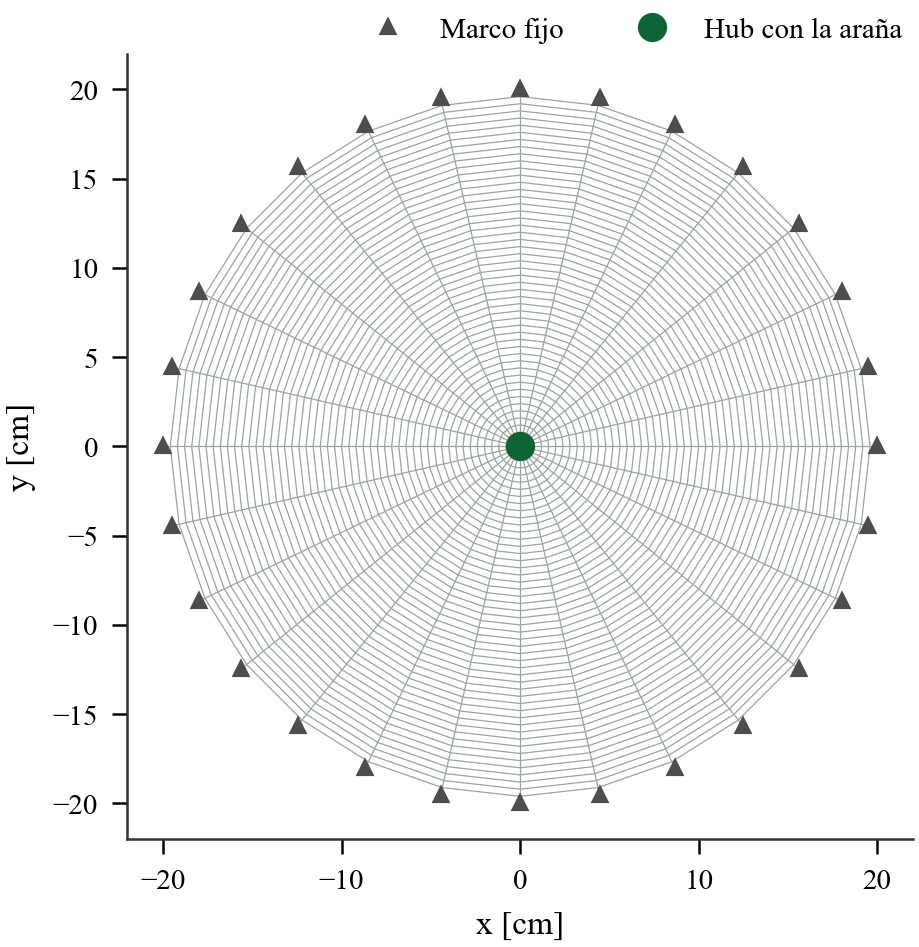
\includegraphics[width=0.58\textwidth]{figuras/fig01_geometria.png}
\caption{Geometría discretizada de la configuración base utilizada en el análisis modal.}
\label{fig:geometria}
\end{figure}

Como control de consistencia, la implementación evalúa la simetría de la rigidez las relaciones de ortogonalidad de la ecuación~\eqref{eq:ortogonalidad}. La Tabla~\ref{tab:verificacion} presenta los indicadores obtenidos en la ejecución actual. El bloque de acoplamiento entre los grados $x$--$y$ y $z$ resultó exactamente nulo en precisión numérica. Los residuos modales se mantienen por debajo de $10^{-9}$ y los errores de ortogonalidad respecto a $\mathbf M$ son del orden de la precisión de máquina. Estos valores verifican la consistencia algebraica del solucionador.

\begin{table}[H]
\centering
\small
\caption{Verificaciones numéricas del análisis modal.}
\label{tab:verificacion}
\begin{tabular}{@{}lcc@{}}
\toprule
Indicador & Modos transversales & Modos en el plano \\
\midrule
Residuo relativo máximo & $6.04\times10^{-11}$ & $8.26\times10^{-10}$ \\
Error en $\boldsymbol{\Phi}^{\mathsf T}\mathbf M\boldsymbol{\Phi}$ & $4.44\times10^{-16}$ & $4.71\times10^{-16}$ \\
Error en $\boldsymbol{\Phi}^{\mathsf T}\mathbf K\boldsymbol{\Phi}$ & $4.08\times10^{-14}$ & $8.24\times10^{-11}$ \\
\bottomrule
\end{tabular}
\end{table}

\section{Resultados obtenidos}

La Tabla~\ref{tab:frecuencias} presenta las primeras seis frecuencias de cada familia junto con su número de onda azimutal dominante $p$. En la familia transversal aparece un primer modo de 2.554~Hz con $p=0$, seguido por un modo axisimétrico de 114.787~Hz y por pares de frecuencias repetidas. En la familia plana, las dos primeras frecuencias son iguales a 65.577~Hz y tienen $p=1$. La repetición de frecuencias no constituye un error numérico; corresponde a modos degenerados asociados con la simetría circular discreta de la estructura.

\begin{table}[H]
\centering
\small
\caption{Primeras frecuencias naturales y número de onda azimutal dominante.}
\label{tab:frecuencias}
\begin{tabular}{@{}ccc|ccc@{}}
\toprule
\multicolumn{3}{c|}{Transversales} & \multicolumn{3}{c}{En el plano}\\
Modo & $f$ [Hz] & $p$ & Modo & $f$ [Hz] & $p$ \\
\midrule
1 & 2.554 & 0 & 1 & 65.577 & 1 \\
2 & 114.787 & 0 & 2 & 65.577 & 1 \\
3 & 130.265 & 1 & 3 & 130.265 & 0 \\
4 & 130.265 & 1 & 4 & 146.797 & 1 \\
5 & 162.003 & 2 & 5 & 146.797 & 1 \\
6 & 162.003 & 2 & 6 & 181.013 & 2 \\
\bottomrule
\end{tabular}
\end{table}

La Figura~\ref{fig:espectro} presenta el espectro modal en escala logarítmica. El panel izquierdo compara las primeras 24 frecuencias de ambas familias, mientras que el panel derecho muestra los 1373 modos transversales calculados. La separación entre la primera frecuencia transversal y el resto del espectro es evidente. La Figura~\ref{fig:p} reorganiza las frecuencias de acuerdo con el número azimutal dominante $p$ definido en la ecuación~\eqref{eq:dft_angular}; esta representación permite visualizar la estructura de familias asociada a la simetría rotacional.

\begin{figure}[H]
\centering
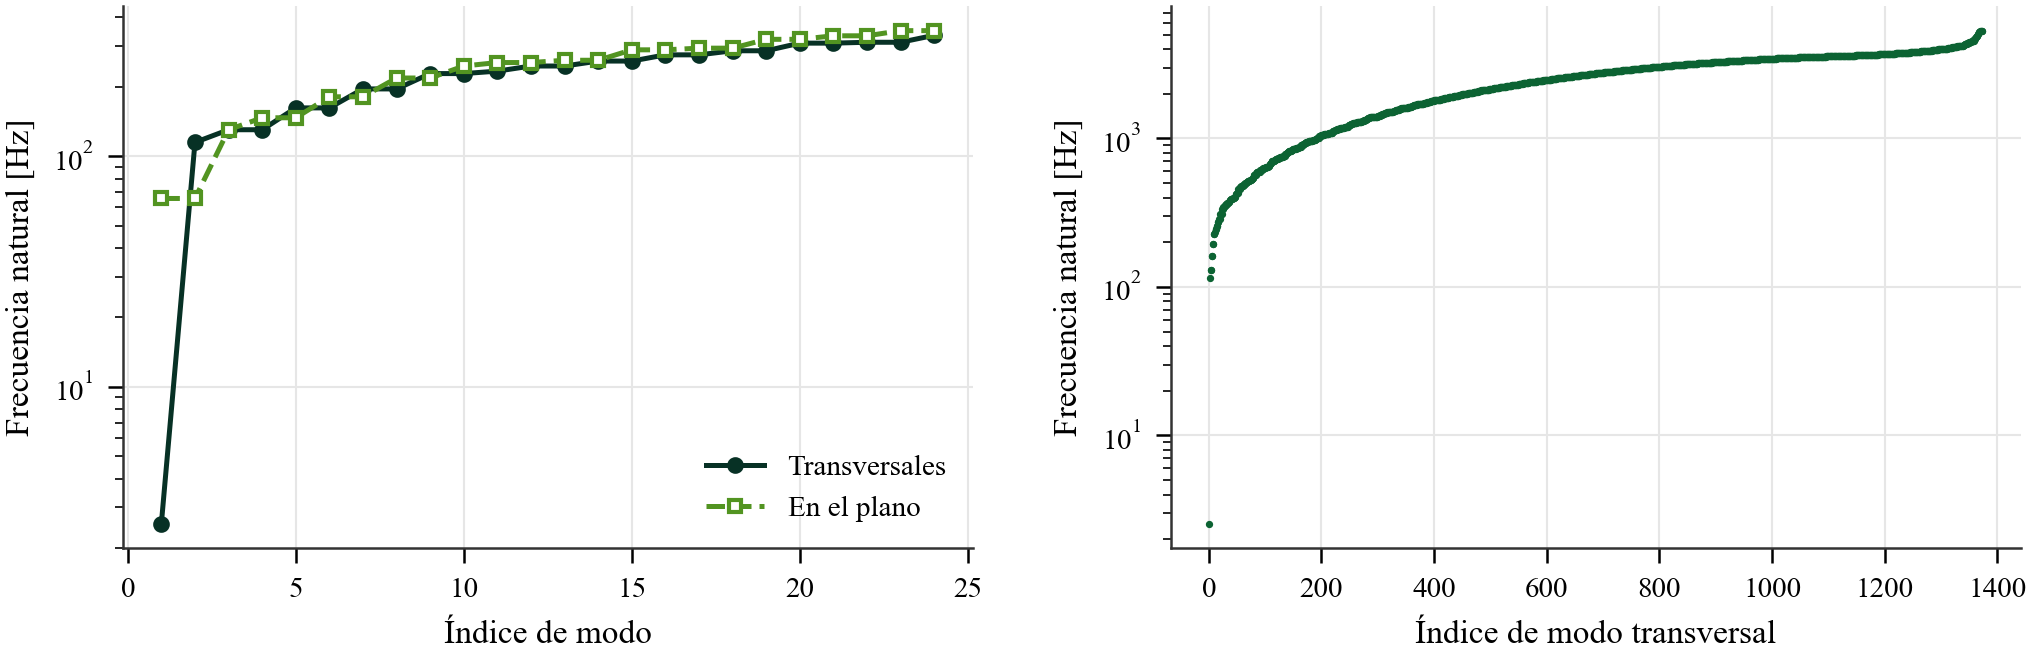
\includegraphics[width=0.97\textwidth]{figuras/fig02_espectro_modal.png}
\caption{Espectro de frecuencias naturales. A la izquierda se comparan los primeros 24 modos transversales y en el plano; a la derecha se muestra el espectro transversal completo.}
\label{fig:espectro}
\end{figure}

\begin{figure}[H]
\centering
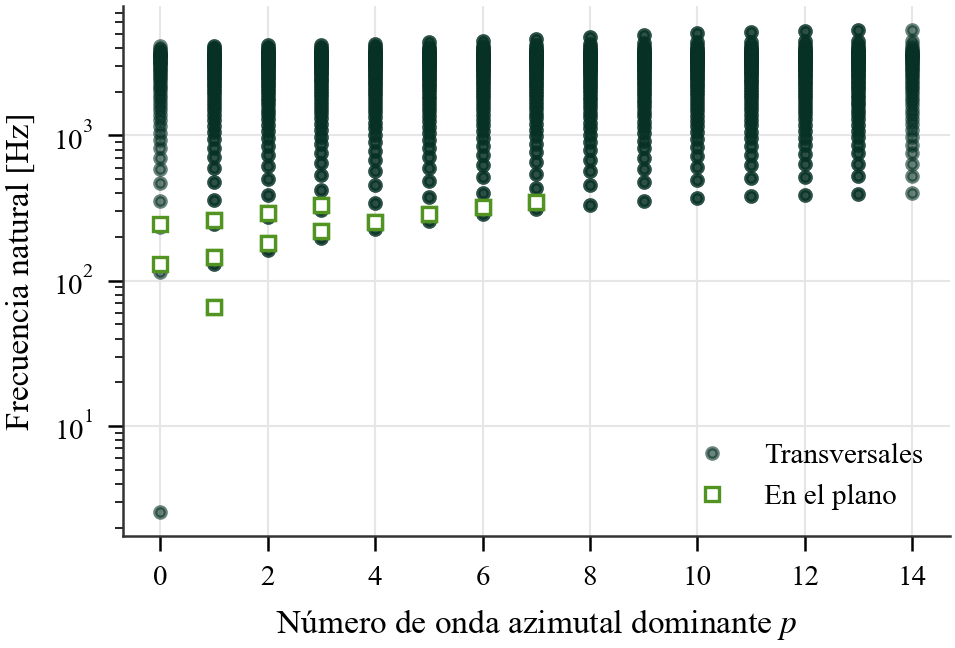
\includegraphics[width=0.69\textwidth]{figuras/fig03_frecuencia_vs_p.png}
\caption{Clasificación de las frecuencias naturales mediante el número de onda azimutal dominante $p$.}
\label{fig:p}
\end{figure}

La Figura~\ref{fig:modosT} muestra las primeras seis formas modales transversales. El color representa la amplitud modal relativa en la dirección $z$, normalizada de manera independiente para cada modo. El primer modo presenta la frecuencia más baja y una participación dominante del hub, mientras que los modos siguientes desarrollan patrones espaciales sobre los anillos. Los modos 3 y 4 comparten la frecuencia de 130.265~Hz y $p=1$; los modos 5 y 6 comparten 162.003~Hz y $p=2$. Cada par corresponde a dos orientaciones angulares independientes de una misma familia de simetría.

\begin{figure}[H]
\centering
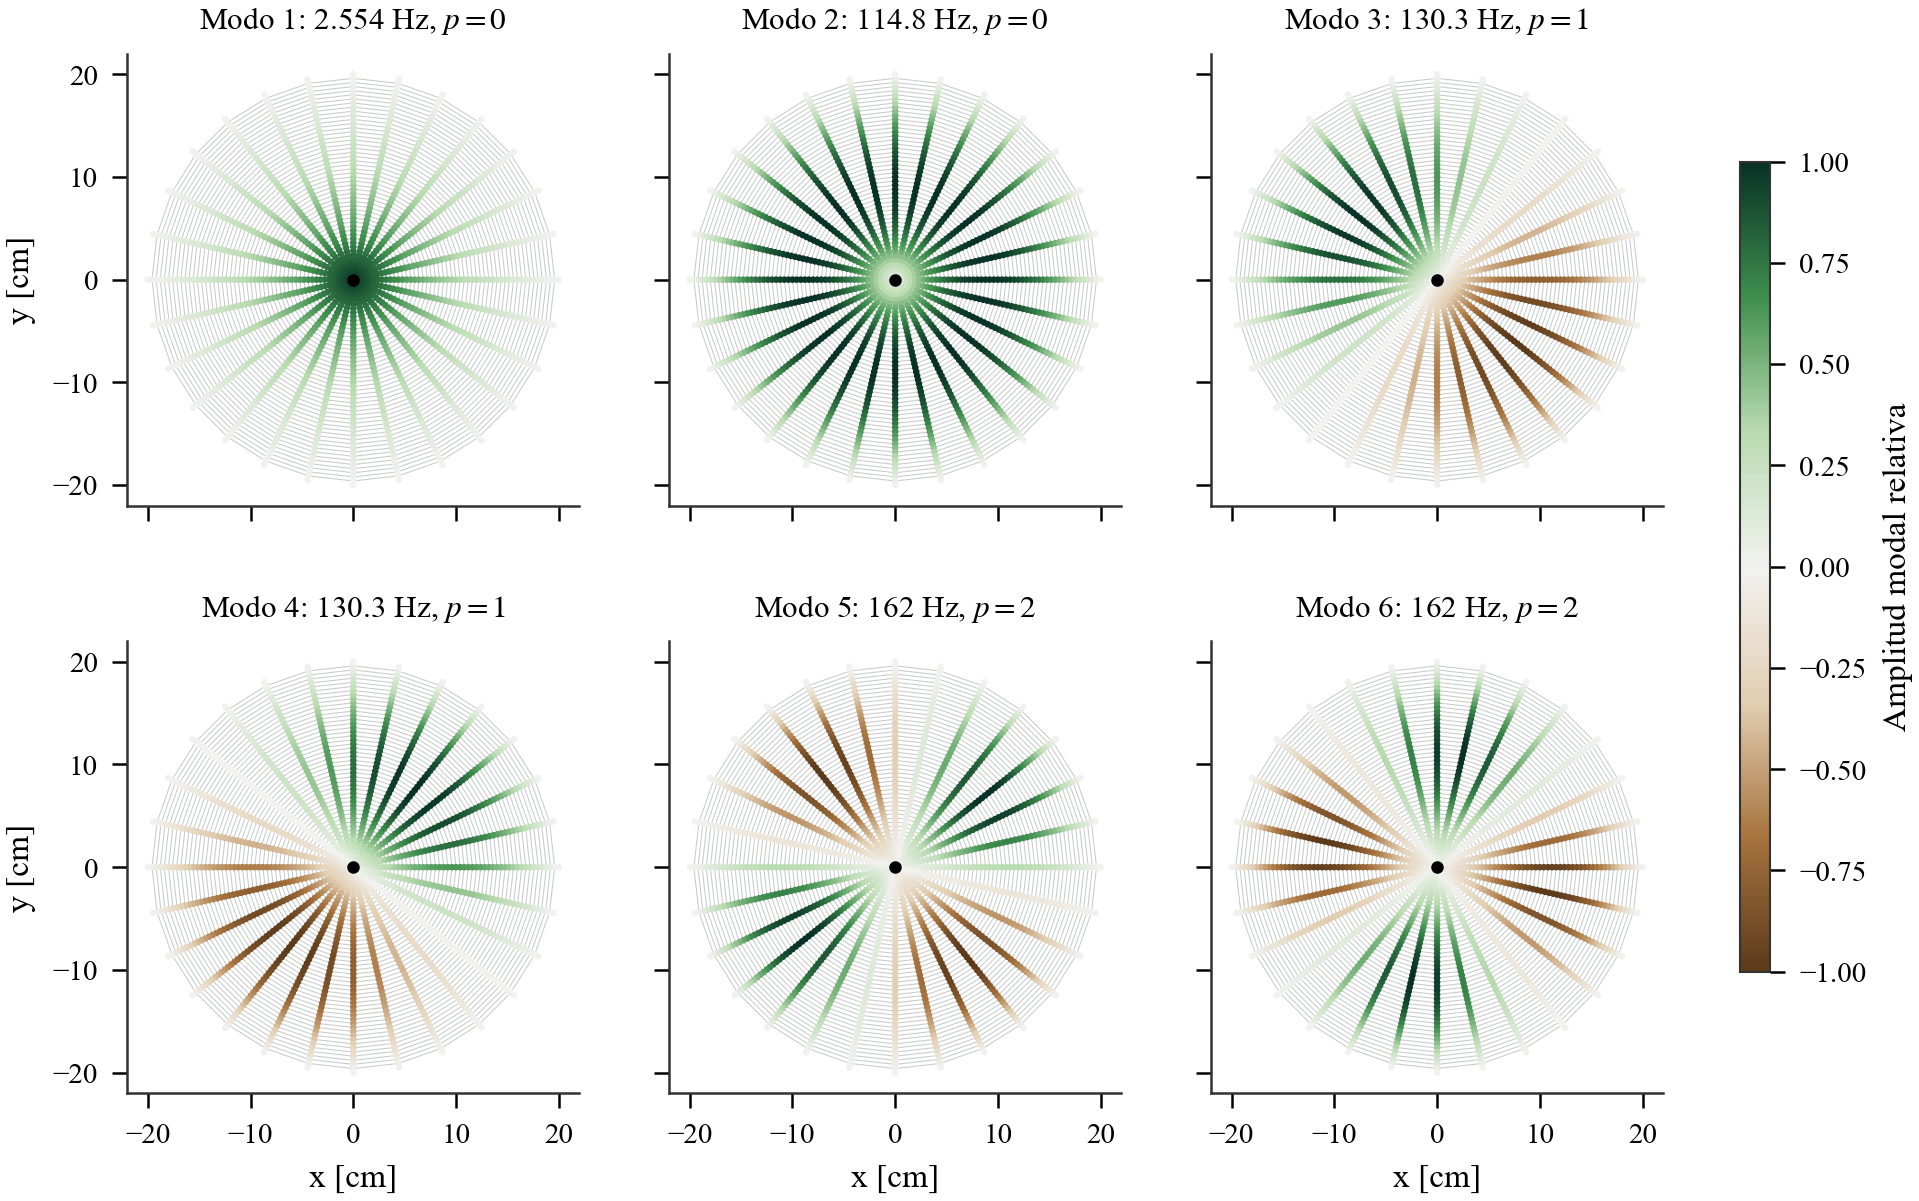
\includegraphics[width=0.96\textwidth]{figuras/fig04_modos_transversales.png}
\caption{Primeros seis modos transversales. El color indica la amplitud modal relativa de la componente $z$.}
\label{fig:modosT}
\end{figure}

La Figura~\ref{fig:modosP} presenta los seis primeros modos en el plano. Las flechas representan las componentes $(u_x,u_y)$ y permiten distinguir patrones que no pueden observarse únicamente a partir del valor de la frecuencia. Los dos primeros modos forman un par degenerado de 65.577~Hz con $p=1$, mientras que el tercer modo es axisimétrico en la clasificación azimutal y aparece a 130.265~Hz.

\begin{figure}[H]
\centering
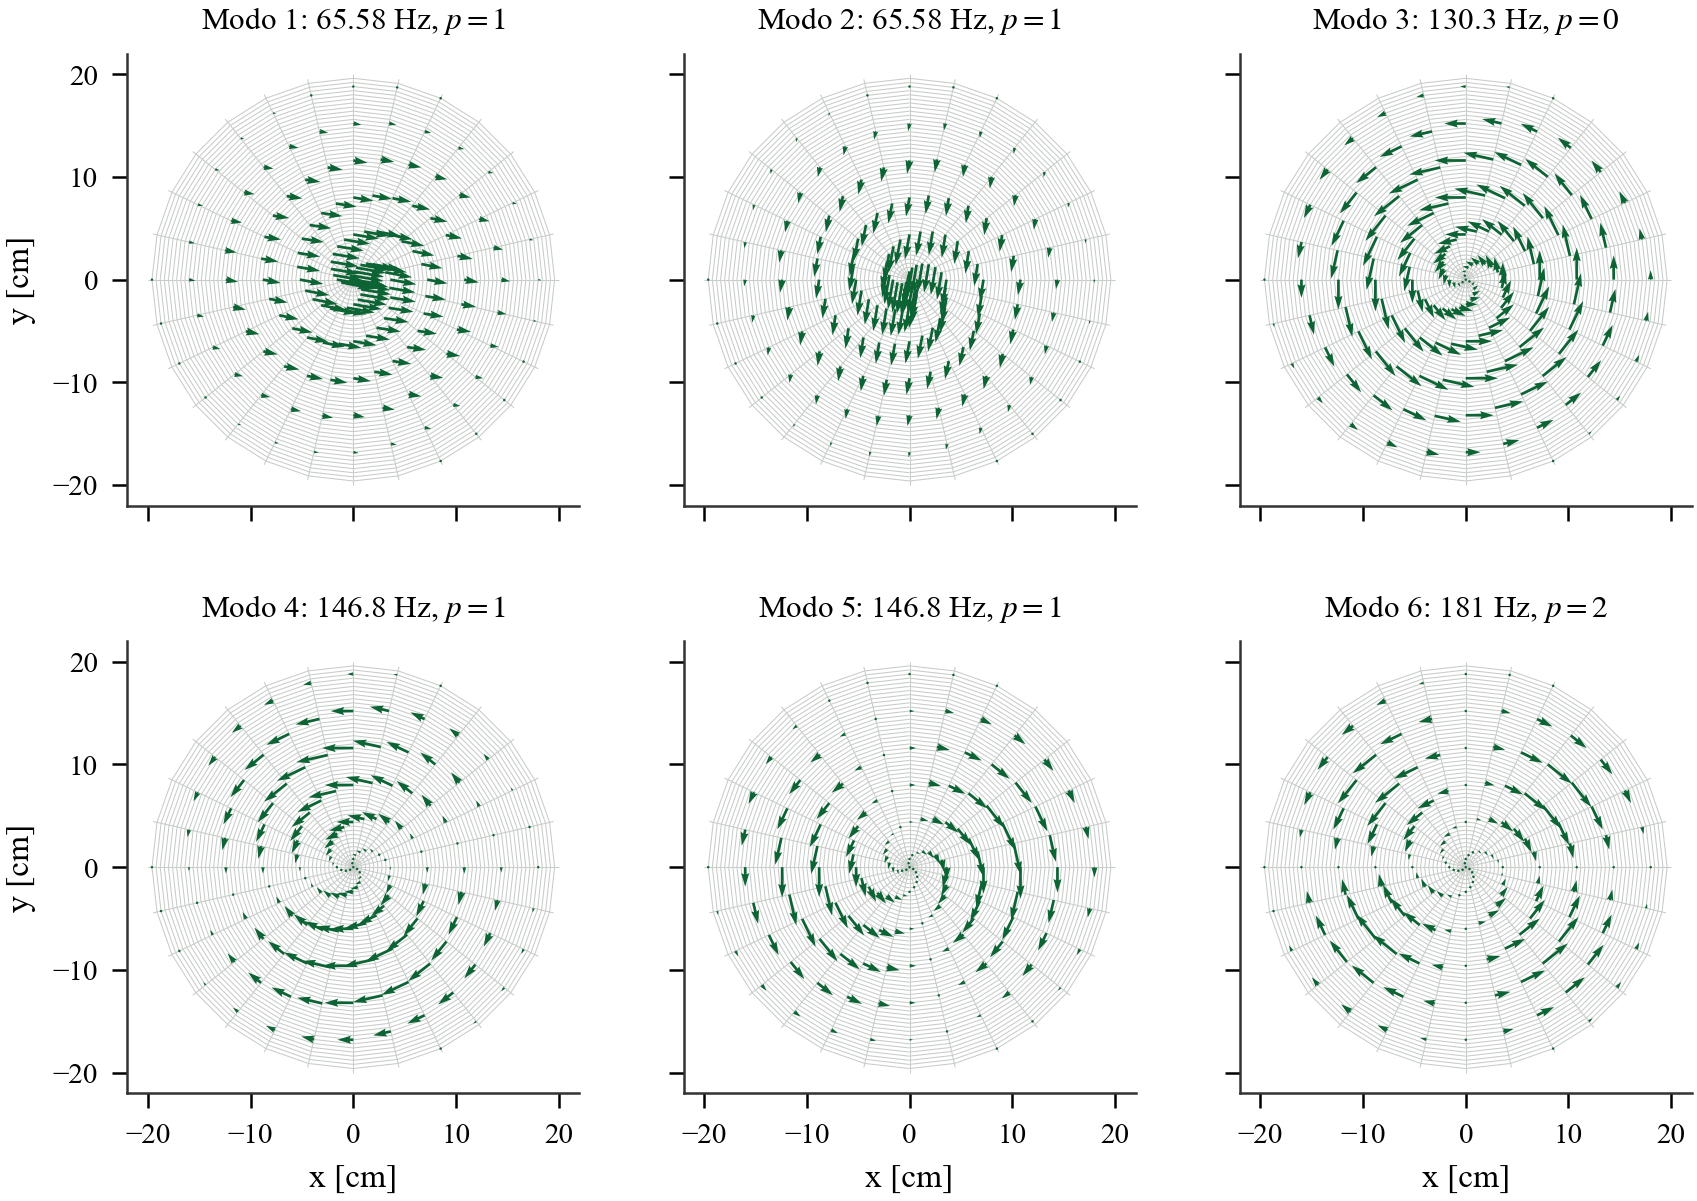
\includegraphics[width=0.96\textwidth]{figuras/fig05_modos_plano.png}
\caption{Primeros seis modos en el plano. Las flechas representan la dirección y amplitud relativa del desplazamiento modal $(u_x,u_y)$.}
\label{fig:modosP}
\end{figure}

La Figura~\ref{fig:masa_perfiles} sintetiza dos resultados que ayudan a interpretar la familia transversal. La comparación con y sin masa de araña muestra que la masa concentrada introduce un modo de muy baja frecuencia: el primer valor pasa de 74.892~Hz sin la araña a 2.554~Hz cuando se incluyen los 50~mg en el hub. En cambio, los perfiles radiales muestran cómo se distribuye la amplitud RMS de cada modo a medida que aumenta el radio. El modo 1 decrece desde el centro hacia el marco, mientras que el modo 2 presenta un máximo en una región intermedia. Los modos 3 y 4 tienen exactamente el mismo perfil radial RMS; por esta razón sus curvas se superponen en el panel derecho y la curva dibujada en último lugar oculta visualmente a la otra, aunque las formas modales completas sí difieren en su orientación angular.

\begin{figure}[H]
\centering
\begin{subfigure}[t]{0.49\textwidth}
\centering
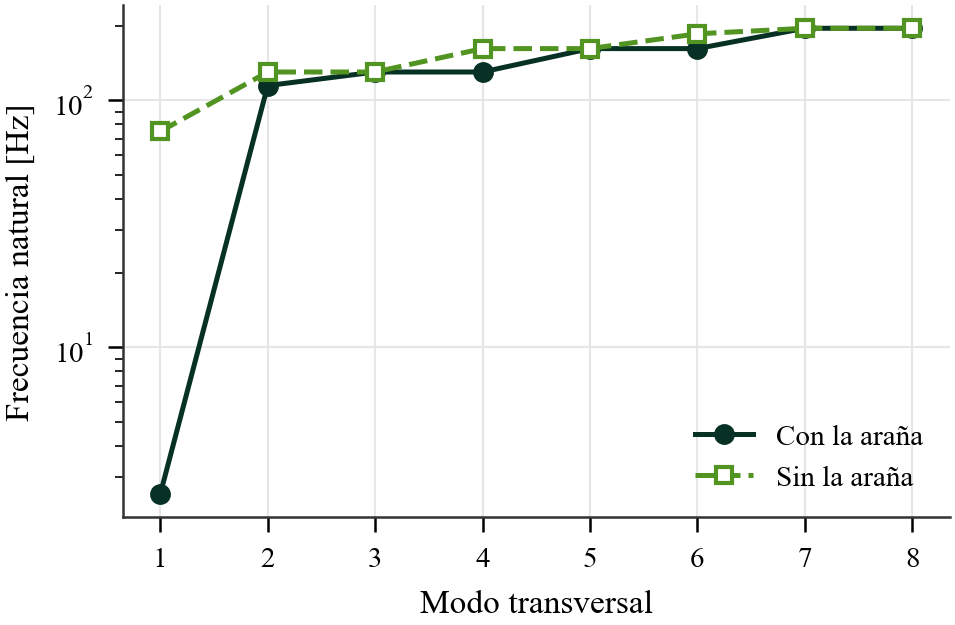
\includegraphics[width=\linewidth]{figuras/fig06_comparacion_masa_arana.png}
\caption{Primeras frecuencias transversales con y sin la masa de la araña.}
\end{subfigure}\hfill
\begin{subfigure}[t]{0.49\textwidth}
\centering
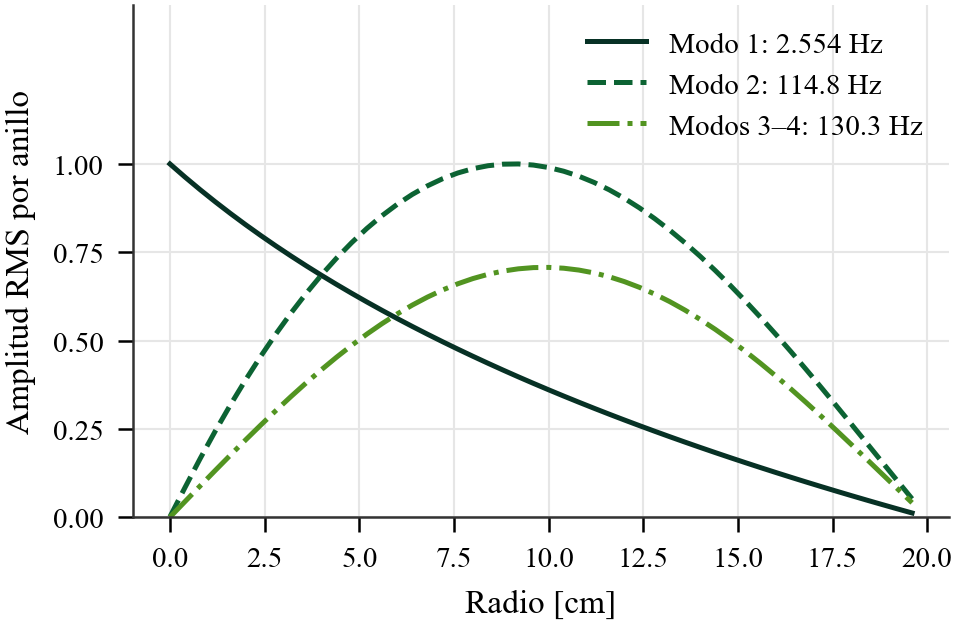
\includegraphics[width=\linewidth]{figuras/fig07_perfiles_radiales.png}
\caption{Perfil radial RMS de los primeros cuatro modos transversales.}
\end{subfigure}
\caption{Efecto de la masa concentrada y distribución radial de los modos transversales.}
\label{fig:masa_perfiles}
\end{figure}

\section{Análisis y discusión de resultados}

El resultado modal más destacado es la aparición de una frecuencia transversal de 2.554~Hz cuando se incluye la masa de la araña. La forma modal de la Figura~\ref{fig:modosT} y el panel (b) de la Figura~\ref{fig:masa_perfiles} muestran que este modo está fuertemente asociado con el movimiento del hub. La comparación del panel (a) de la Figura~\ref{fig:masa_perfiles} confirma que este comportamiento depende de la masa concentrada, pues al retirarla la primera frecuencia de la estructura asciende a 74.892~Hz. Por tanto, la presencia de la araña no puede tratarse como una modificación despreciable si se desea estudiar la dinámica de baja frecuencia.

La segunda característica importante es la degeneración modal. En una red con simetría cíclica, los patrones angulares con $p>0$ pueden representarse mediante dos combinaciones independientes equivalentes a componentes seno y coseno. Esto explica que los modos 3 y 4 transversales tengan la misma frecuencia y el mismo número $p=1$, y que los modos 5 y 6 hagan lo mismo para $p=2$. La degeneración se observa también en la familia plana. La coincidencia de los perfiles radiales de los modos 3 y 4 en el panel (b) de la Figura~\ref{fig:masa_perfiles} es una consecuencia directa de este hecho: al reducir una forma bidimensional a una medida RMS por anillo se elimina la información de fase angular que permite distinguir a los dos miembros del par.

La separación exacta entre modos transversales y modos en el plano es coherente con la geometría de referencia. Debido a que todos los hilos están inicialmente contenidos en $z=0$, la linealización no genera términos $xz$ ni $yz$ en la matriz elemental. El valor nulo del bloque de acoplamiento obtenido numéricamente constituye una comprobación directa de esta propiedad. Esta separación también permite interpretar físicamente la contribución de la pretensión: en la familia transversal, la rigidez proviene principalmente del término geométrico $T_{ij}^{0}/L_{ij}^{0}$ de la ecuación~\eqref{eq:ke}, mientras que los movimientos dentro del plano contienen además una contribución axial importante.

Los resultados actuales deben entenderse como una caracterización modal de la configuración base y no todavía como una respuesta completa a la pregunta general del proyecto. Para establecer cómo la geometría controla la transmisión de una perturbación será necesario introducir el forzamiento temporal, implementar la superposición modal o la integral de Duhamel, calcular la receptancia entre nodos y posteriormente repetir el análisis para diferentes valores de $N$, $M$ y distribución radial. El análisis modal desarrollado en esta etapa proporciona la base necesaria para esas extensiones, porque fija las frecuencias, formas modales y relaciones de ortogonalidad que se utilizarán en la respuesta forzada.

\section{Estado de la implementación numérica}

La Tabla~\ref{tab:estado} resume el estado técnico del desarrollo. La construcción de la red, el ensamblaje de matrices y el análisis modal se consideran cerrados para la configuración base en el sentido de que ya cuentan con una implementación funcional y verificaciones numéricas. La respuesta dinámica temporal y la transmisión entre nodos permanecen pendientes en la versión actual del proyecto. Las figuras de respuesta impulsional, transferencia y mapas de transmisión producidas en versiones anteriores se conservan en el material de referencia del proyecto, pero no se utilizan en este informe como evidencia de resultados actuales porque esas rutinas todavía no forman parte del código modular validado.

\begin{table}[H]
\centering
\small
\caption{Estado técnico de la implementación numérica.}
\label{tab:estado}
\begin{tabularx}{0.96\textwidth}{@{}X p{2.5cm} X@{}}
\toprule
Componente & Estado & Alcance actual \\
\midrule
Geometría, conectividad y pretensiones & Completado & Red base con marco fijo y hub libre \\
Masas nodales y matrices $\mathbf M$ y $\mathbf K$ & Completado & Ensamblaje y verificaciones estructurales \\
Análisis modal & Completado & Espectro transversal completo y 24 primeros modos planos \\
Clasificación azimutal y verificaciones & Completado & Número $p$, residuos y ortogonalidad \\
Comparación con y sin masa de la araña & Completado & Primeros ocho modos de ambas familias \\
Respuesta temporal impulsional & Pendiente & Requiere superposición modal y definición del forzamiento \\
Función de transferencia e índice de transmisión & Pendiente & Se implementará después de la respuesta temporal \\
Variación de configuraciones geométricas & Pendiente & Comparación sistemática de $N$, $M$ y radios \\
Análisis global y conclusiones finales & Pendiente & Depende de las simulaciones comparativas \\
\bottomrule
\end{tabularx}
\end{table}

\section{Conclusiones}
El modelo matemático propuesto permite obtener tanto modos de vibración en el plano como transversales para una telaraña con y sin la masa de la araña.La implementación realizada presenta una buena consistencia algebraica con el modelo desarrollado, como lo muestran las verificaciones numéricas de los residuos y las relaciones de ortogonalidad.

Adicionalmente, se encontró que,  para la geometría plana y el modelo linealizado considerados, no existe acoplamiento entre los movimientos transversales y los movimientos en el plano, por lo que ambas familias pueden estudiarse de manera independiente. Además, se observaron frecuencias naturales repetidas, como consecuencia de la simetría de la estructura.

Por último, se observó que la presencia de la araña modifica significativamente el comportamiento vibratorio transversal, especialmente el primer modo, cuya frecuencia disminuye de 74.892 Hz a 2.554 Hz al incorporar la masa central.

Aunque los resultados obtenidos constituyen una catacterización del comportamiento modal de la telaraña, como trabajo futuro aún es necesario analizar la respuesta de la red ante perturbaciones externas y estudiar cómo cambia al modificar su geometría, con el fin de responder al objetivo principal del proyecto.

\FloatBarrier
\footnotesize\begin{thebibliography}{99}

\bibitem{masters1981} W. M. Masters and H. Markl, ``Vibration signal transmission in spider orb webs,'' \textit{Science}, vol. 213, no. 4505, pp. 363--365, 1981.

\bibitem{mortimer2016} B. Mortimer, A. Soler, C. R. Siviour, R. Zaera, and F. Vollrath, ``Tuning the instrument: sonic properties in the spider's web,'' \textit{Journal of the Royal Society Interface}, vol. 13, no. 122, 20160341, 2016.

\bibitem{mortimer2019} B. Mortimer, ``A Spider's Vibration Landscape: Adaptations to Promote Vibrational Information Transfer in Orb Webs,'' \textit{Integrative and Comparative Biology}, vol. 59, no. 6, pp. 1636--1645, 2019.

\bibitem{nakata2010} K. Nakata, ``Attention focusing in a sit-and-wait forager: a spider controls its prey-detection ability in different web sectors by adjusting thread tension,'' \textit{Proceedings of the Royal Society B}, vol. 277, pp. 29--33, 2010.

\bibitem{aoyanagi2010} Y. Aoyanagi and K. Okumura, ``Simple Model for the Mechanics of Spider Webs,'' \textit{Physical Review Letters}, vol. 104, 038102, 2010.

\bibitem{lott2022} M. Lott, V. F. Dal Poggetto, G. Greco, N. M. Pugno, and F. Bosia, ``Prey localization in spider orb webs using modal vibration analysis,'' \textit{Scientific Reports}, vol. 12, 19045, 2022.

\bibitem{soler2016} A. Soler and R. Zaera, ``The secondary frame in spider orb webs: the detail that makes the difference,'' \textit{Scientific Reports}, vol. 6, 31265, 2016.

\bibitem{meirovitch2001} L. Meirovitch, \textit{Fundamentals of Vibrations}. McGraw-Hill, 2001.

\bibitem{jayaraman1981} H. B. Jayaraman and W. C. Knudson, ``A curved element for the analysis of cable structures,'' \textit{Computers \& Structures}, vol. 14, no. 3--4, pp. 325--333, 1981.

\bibitem{inman2014} D. J. Inman, \textit{Engineering Vibration}, 4th ed. Pearson, 2014.

\bibitem{ewins2000} D. J. Ewins, \textit{Modal Testing: Theory, Practice and Application}, 2nd ed. Research Studies Press, 2000.

\bibitem{yavuz2024} K. Yavuz, A. M. Soler, R. Zaera, and S. Jahangirov, ``Effect of spider's weight on signal transmittance in vertical orb webs,'' \textit{Royal Society Open Science}, vol. 11, 240986, 2024.

\bibitem{stauffer1994} S. L. Stauffer, S. L. Coguill, and R. V. Lewis, ``Comparison of physical properties of three silks from \textit{Nephila clavipes} and \textit{Araneus gemmoides},'' \textit{Journal of Arachnology}, vol. 22, pp. 5--11, 1994.

\bibitem{gosline1999} J. M. Gosline, P. A. Guerette, C. S. Ortlepp, and K. N. Savage, ``The mechanical design of spider silks: from fibroin sequence to mechanical function,'' \textit{Journal of Experimental Biology}, vol. 202, no. 23, pp. 3295--3303, 1999.

\end{thebibliography}

\end{document}
